\documentclass[tikz,border=10pt]{standalone}
\usepackage{lmodern}        % Latin Modern fonts - prevents font warnings
\usepackage[T1]{fontenc}    % Proper font encoding
\usepackage{tikz}
\usepackage{xcolor}
\usetikzlibrary{shapes.geometric,arrows.meta,positioning,fit,patterns,calc,matrix}

\definecolor{userspace}{RGB}{173,216,230}
\definecolor{kernelspace}{RGB}{255,165,79}
\definecolor{cpuhw}{RGB}{169,169,169}
\definecolor{datastructure}{RGB}{144,238,144}

\begin{document}
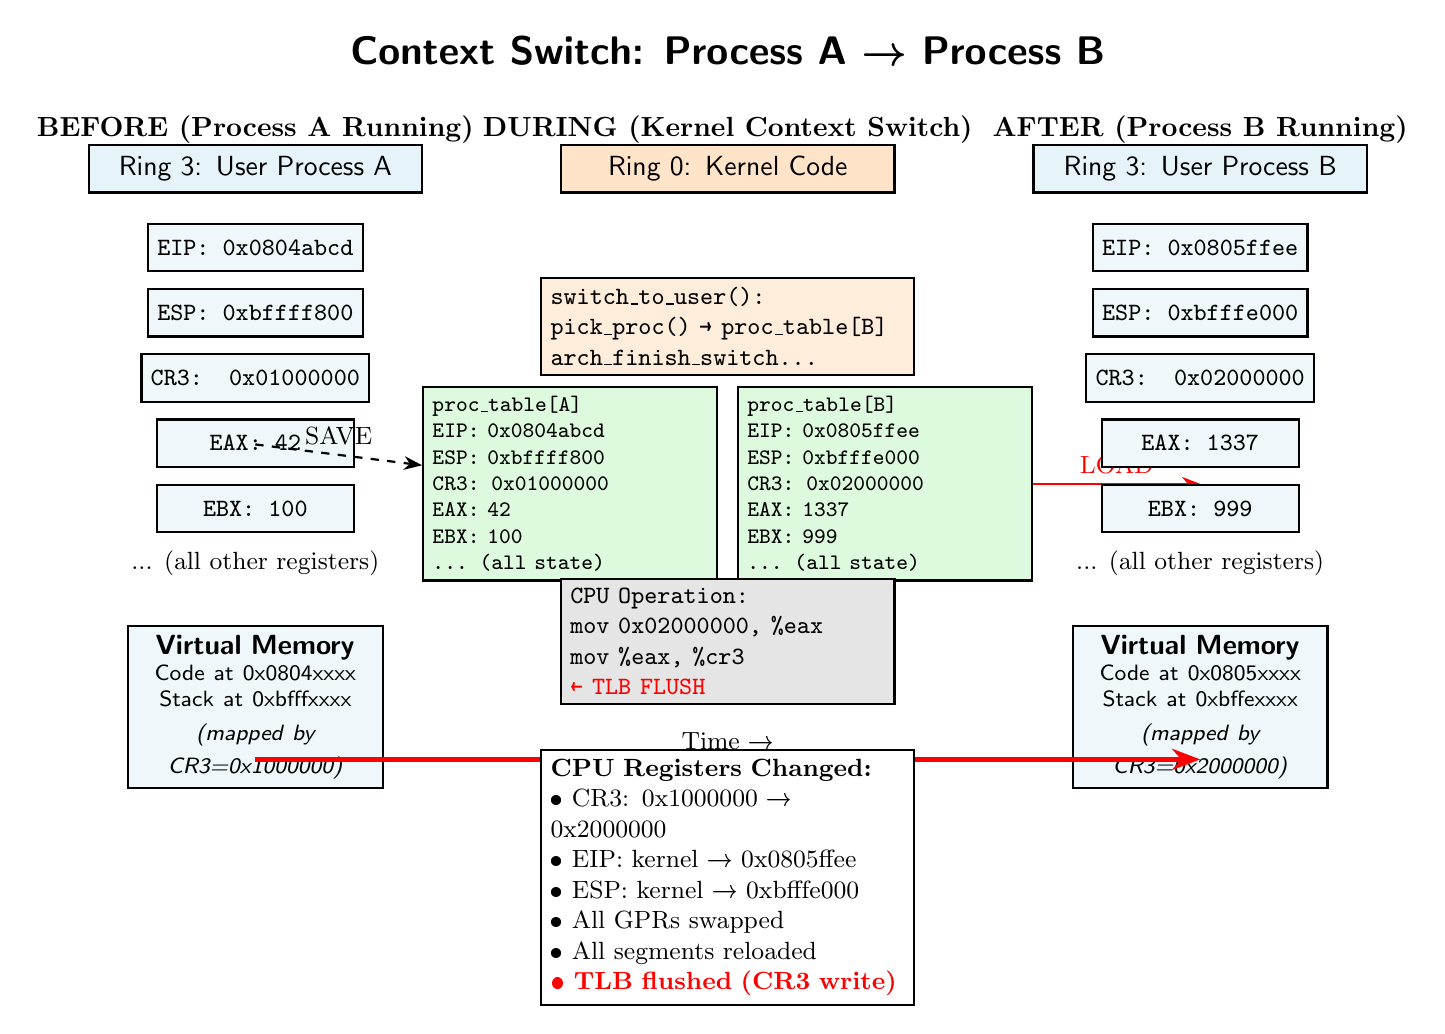
\begin{tikzpicture}[
    node distance=0.5cm,
    every node/.style={font=\sffamily},
    box/.style={rectangle, draw, thick, minimum width=2.5cm, minimum height=0.6cm},
    regbox/.style={box, font=\ttfamily\small},
    arrow/.style={-Stealth, thick},
]

% Title
\node[font=\sffamily\Large\bfseries] at (8, 11) {Context Switch: Process A → Process B};

% --- BEFORE PANEL ---
\node[font=\bfseries] at (2, 10) {BEFORE (Process A Running)};
\node[box, fill=userspace!30, text width=4cm, align=center] (before_label) at (2, 9.5) {Ring 3: User Process A};

% Process A registers
\node[regbox, fill=userspace!20] (a_eip) at (2, 8.5) {EIP: 0x0804abcd};
\node[regbox, fill=userspace!20, below=0.2cm of a_eip] (a_esp) {ESP: 0xbffff800};
\node[regbox, fill=userspace!20, below=0.2cm of a_esp] (a_cr3) {CR3: 0x01000000};
\node[regbox, fill=userspace!20, below=0.2cm of a_cr3] (a_eax) {EAX: 42};
\node[regbox, fill=userspace!20, below=0.2cm of a_eax] (a_ebx) {EBX: 100};
\node[font=\small, below=0.1cm of a_ebx] (a_more) {... (all other registers)};

% Memory layout A
\node[box, fill=userspace!20, text width=3cm, minimum height=1.5cm, align=center, below=0.5cm of a_more] (mem_a) {
    \textbf{Virtual Memory}\\
    \footnotesize
    Code at 0x0804xxxx\\
    Stack at 0xbfffxxxx\\
    \textit{(mapped by CR3=0x1000000)}
};

% --- DURING PANEL ---
\node[font=\bfseries] at (8, 10) {DURING (Kernel Context Switch)};
\node[box, fill=kernelspace!30, text width=4cm, align=center] (during_label) at (8, 9.5) {Ring 0: Kernel Code};

% Kernel code flow
\node[box, fill=kernelspace!20, text width=4.5cm, align=left, font=\ttfamily\small] at (8, 7.5) {
    \textbf{switch\_to\_user():}\\
    pick\_proc() → proc\_table[B]\\
    arch\_finish\_switch...
};

% Process table A
\node[box, fill=datastructure!30, text width=3.5cm, align=left, font=\ttfamily\footnotesize] (pt_a) at (6, 5.5) {
    \textbf{proc\_table[A]}\\
    EIP: 0x0804abcd\\
    ESP: 0xbffff800\\
    CR3: 0x01000000\\
    EAX: 42\\
    EBX: 100\\
    ... (all state)
};

% Process table B
\node[box, fill=datastructure!30, text width=3.5cm, align=left, font=\ttfamily\footnotesize] (pt_b) at (10, 5.5) {
    \textbf{proc\_table[B]}\\
    EIP: 0x0805ffee\\
    ESP: 0xbfffe000\\
    CR3: 0x02000000\\
    EAX: 1337\\
    EBX: 999\\
    ... (all state)
};

% Critical CR3 operation
\node[box, fill=cpuhw!30, text width=4cm, align=left, font=\ttfamily\small] (cr3_op) at (8, 3.5) {
    \textbf{CPU Operation:}\\
    mov 0x02000000, \%eax\\
    mov \%eax, \%cr3\\
    \textcolor{red}{\textbf{← TLB FLUSH}}
};

% Arrows showing save and load
\draw[arrow, dashed] (2, 6) -- (pt_a) node[midway, above, font=\small] {SAVE};
\draw[arrow, thick, color=red] (pt_b) -- (14, 5.5) node[midway, above, font=\small, color=red] {LOAD};

% --- AFTER PANEL ---
\node[font=\bfseries] at (14, 10) {AFTER (Process B Running)};
\node[box, fill=userspace!30, text width=4cm, align=center] (after_label) at (14, 9.5) {Ring 3: User Process B};

% Process B registers
\node[regbox, fill=userspace!20] (b_eip) at (14, 8.5) {EIP: 0x0805ffee};
\node[regbox, fill=userspace!20, below=0.2cm of b_eip] (b_esp) {ESP: 0xbfffe000};
\node[regbox, fill=userspace!20, below=0.2cm of b_esp] (b_cr3) {CR3: 0x02000000};
\node[regbox, fill=userspace!20, below=0.2cm of b_cr3] (b_eax) {EAX: 1337};
\node[regbox, fill=userspace!20, below=0.2cm of b_eax] (b_ebx) {EBX: 999};
\node[font=\small, below=0.1cm of b_ebx] (b_more) {... (all other registers)};

% Memory layout B
\node[box, fill=userspace!20, text width=3cm, minimum height=1.5cm, align=center, below=0.5cm of b_more] (mem_b) {
    \textbf{Virtual Memory}\\
    \footnotesize
    Code at 0x0805xxxx\\
    Stack at 0xbffexxxx\\
    \textit{(mapped by CR3=0x2000000)}
};

% Main flow arrows
\draw[arrow, ultra thick, color=red] (2, 2) -- (8, 2) -- (14, 2);
\node[above, font=\small] at (8, 2) {Time →};

% Key changes annotation
\node[draw, thick, fill=white, text width=4.5cm, align=left, font=\small] at (8, 0.5) {
    \textbf{CPU Registers Changed:}\\
    • CR3: 0x1000000 → 0x2000000\\
    • EIP: kernel → 0x0805ffee\\
    • ESP: kernel → 0xbfffe000\\
    • All GPRs swapped\\
    • All segments reloaded\\
    \textcolor{red}{\textbf{• TLB flushed (CR3 write)}}
};

\end{tikzpicture}
\end{document}
